\documentclass{beamer}
\usepackage[utf8x]{inputenc}
\usepackage{default}

\title{Artificial Intelligence for Battle Robots\\\small halfweg presentatie}
\author{Jeroen Rooijmans, Maarten Inja and Maarten de Waard}
\institute{UvA}
\usetheme{Warsaw}
\newcommand{\slide}[2]
{
\begin{frame}
\begin{block}{#1} 

#2

\end{block} 
\end{frame}
}
\newcommand{\itemslide}[2]
{
\begin{frame}
\begin{block}{#1} 
\begin{itemize}

#2

\end{itemize}
\end{block} 
\end{frame}
}


\begin{document}
\begin{frame}
\titlepage % TIETENSLIDE!
\end{frame}
\begin{frame}
 \Large\tableofcontents
\end{frame}


%deel 1:


\section*{Halfway}
%deel 2:

\subsection{``Challenges''}
\slide{Integrating other programs}{
Problem:
\begin{itemize}
 \item Weird errors about using right ``classpath''
 \item .bat files
 \item Windows terminal \& linux terminal
 \item Starting RoboCode from our project
\end{itemize}
}

\slide{Integrating other programs}{
Solution:
\begin{itemize}
\item Eclipse
\item Read the api (a lot)
\end{itemize}
}

\slide{Implementing the Genotype}{
Problem:
\begin{enumerate}
\item Designing datastructures that:
\begin{itemize}
\item Adequately stores java code
\item Is easily mutated
\end{itemize}
\end{enumerate}
}
\itemslide{Solution}{
\item have add, remove and change command
\item use an expression tree for the arguments
}

\begin{frame}
\frametitle{Solution of giving random arguments:}
\begin{picture}(0.0,0.0) 
   \put(0.0,-120.0){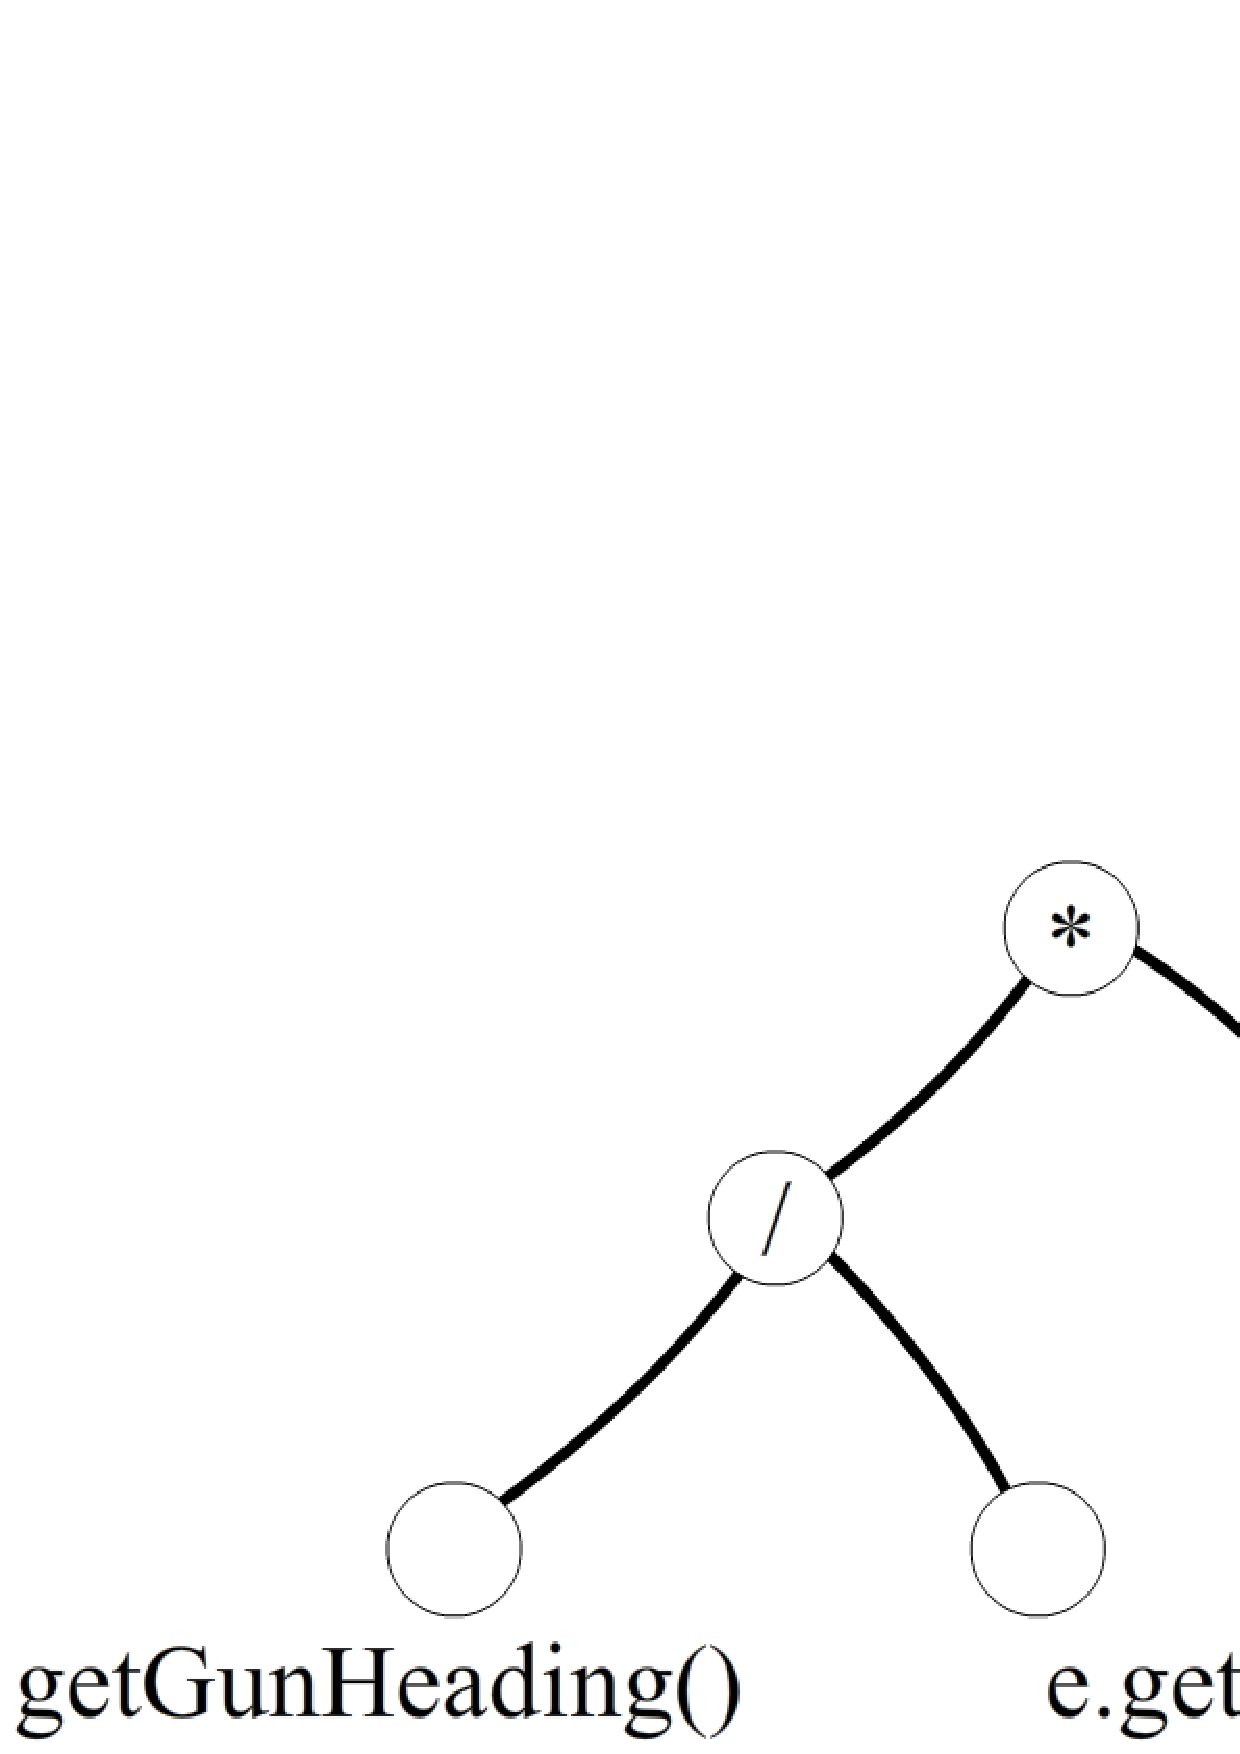
\includegraphics[width=1\textwidth]{tree.png}}
\end{picture}
\end{frame}
\subsection{Progress}
\slide{What can we do now?}{
\begin{itemize}
 \item Create our first generation of bots
 \item Convert genotype to fenotype
 \item Access JGAP and Robocode from our own java code
 \item test our bots with our ``fitness function''
\end{itemize}
}
\subsection{Planning}
\begin{frame}
\frametitle{new planning}
  \begin{picture}(0.0,0.0) 
     \put(0.0,-100.0){\includegraphics[width=1\textwidth]{planning.png}}
  \end{picture}
\end{frame}
\subsection{demo}

\begin{frame}
 \thispagestyle{empty}
\end{frame}


\end{document}
